\section{System Models}
\textbf{\emph{add sequence diagramm mobile and desktop together}}

\subsection{Use Cases} \label{Use Cases}
\fbox{\parbox{\textwidth}{\label{ocfrank} Frank has sparse knowledge of machine learning. He just discovered “Explorer”. On the website that he views using his laptop, he creates a new account. After logging in, he creates a new workspace by selecting sensors to sample data (e.g., accelerometer). He sets up some simple labels (e.g. swipe right, swipe left). After opening the QR code of the workspace, he can select the action to perform on his phone from the available labels. He can also set the duration for a recorded sample and a countdown that is shown before recording. He performs some simple swipe gestures by moving his phone mid-air. The recorded data is labeled and is pushed to the laptop where he can see the data coming in. With a single click he can build a machine learning model that is then available on his smartphone after scanning it's QR code to classify gestures.}}

\fbox{\parbox{\textwidth}{\label{ocalice} Alice is an engineer at a washing machine company. Alice has been observing that HCSOB washing machines with clogged circulating pumps show an unusual pattern of movement during the washing process (error reference 404). The washing machine is moving in a specific rhythm, which Alice recognizes when she is at the customer’s home. However, Alice would rather make a diagnosis without having to go to the customer. Then she remembers the program "Explorer" which she can use to easily develop machine learning models. With the help of the smartphone acceleration sensors in her cell phone, she and her colleagues record the movement patterns at some of her repair sites. After she has collected enough data, she can use the Explorer program to automatically train and deploy a machine learning model with one click. When a new case comes in, Alice just sends the customer a URL to a website of the Explorer. The customer places his smartphone on the washing machine and the model can determine directly "on the edge" whether error 404 is present. This saves Alice money and time. Alice can order the parts for repair and perform the repair with a single visit.}}

\fbox{\parbox{\textwidth}{\label{oc} Brandon is a body building trainer in a big metropol. He has been training people for many years but the latest Carano Virus hit his business hard as he couldn't assist people anymore. He recently watched an advert about the Explorer app and had this wonderful idea that would allow him train customers remotely and earning money in this difficult times. He opened the Explorer app, made himself an account and created labels for his custom exercise routines. After all, he had developed many creative exercise techniques as an experienced body builder. He sent the QR code to his old students that had mastered his techniques to collect diverse samples. With one simple click, he trained a succesful model with the default options. He contected people and asked them to try his new business model. He sent the link to his model to them and with precise instructions for each exercise. With the help of his trained model, people received a feedback in real time if they were performing the exercise routines correctly. }}

\subsection{Desktop System Model}
\begin{center}
    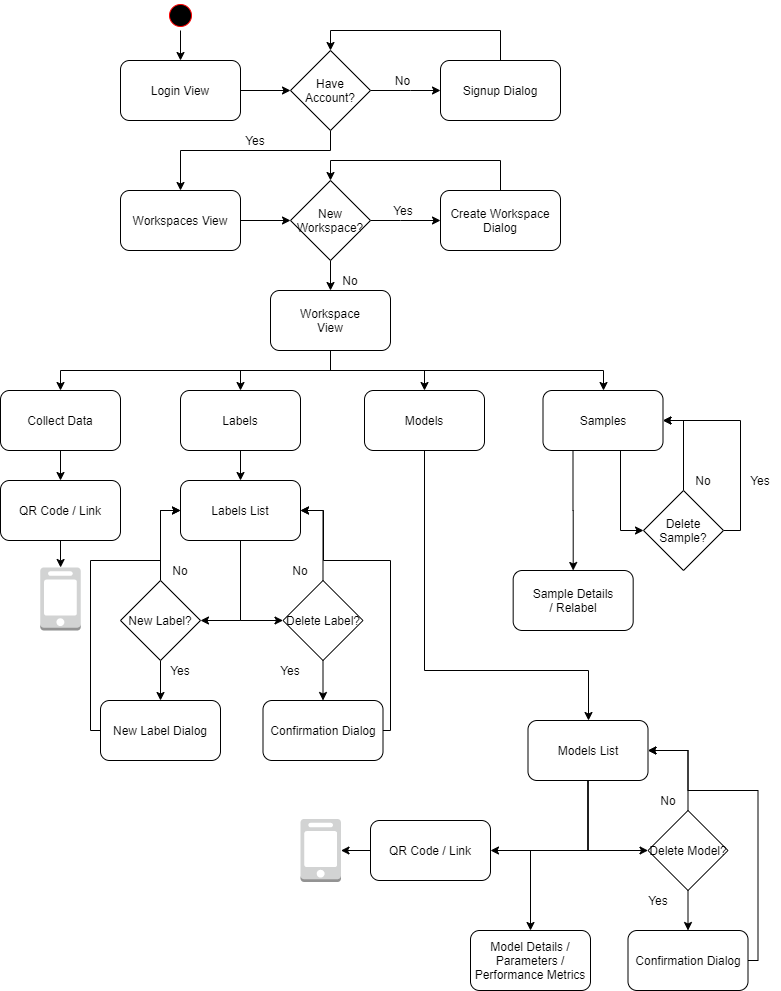
\includegraphics[width=\textwidth,height=0.85\textheight,keepaspectratio]{charts/flow1.png}
\end{center}

\newpage

\subsection{Mobile System Model}
\vspace{1cm}

\begin{figure}[h!]
    \begin{minipage}{0.5\textwidth}
        \centering
        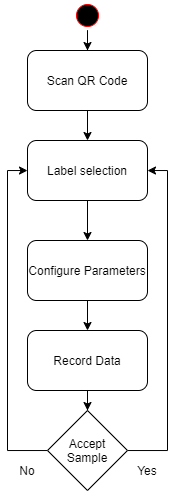
\includegraphics[width=.8\textwidth]{charts/flow2.png}
        \caption{Data Entry}
    \end{minipage}
    \begin{minipage}{0.5\textwidth}
        \centering
        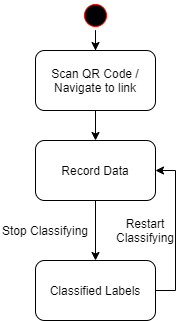
\includegraphics[width=.8\textwidth]{charts/flow3.png}
        \caption{Identification}
    \end{minipage}
\end{figure}